% !TEX root = ./master.tex
 
\section{Results and Discussion}

\subsection{Classification Methods }
We tested several probabilistic classifiers and analyzed the learning curve by randomly sampling. \figref{fig:class} show the accuracy learning curve of logistic regress with L1 and C=1, i.e., {\tt{lr-l1-c1}}, L2 regularization with C=1, and C=10, i.e., {\tt{lr-l2-c1}} and {\tt{lr-l2-c10}}, and multinomial naive babes, i.e., {\tt{mnb}}. We observe that {\tt{mnb}} has the best performance followed by {\tt{lr-l2}} with c=1 and c=10. 

\begin{figure*}[t]
	%\vskip -0.2in
	%\begin{center}
	\centering
		\centerline{
%			\subfigure[IMDB ]{
				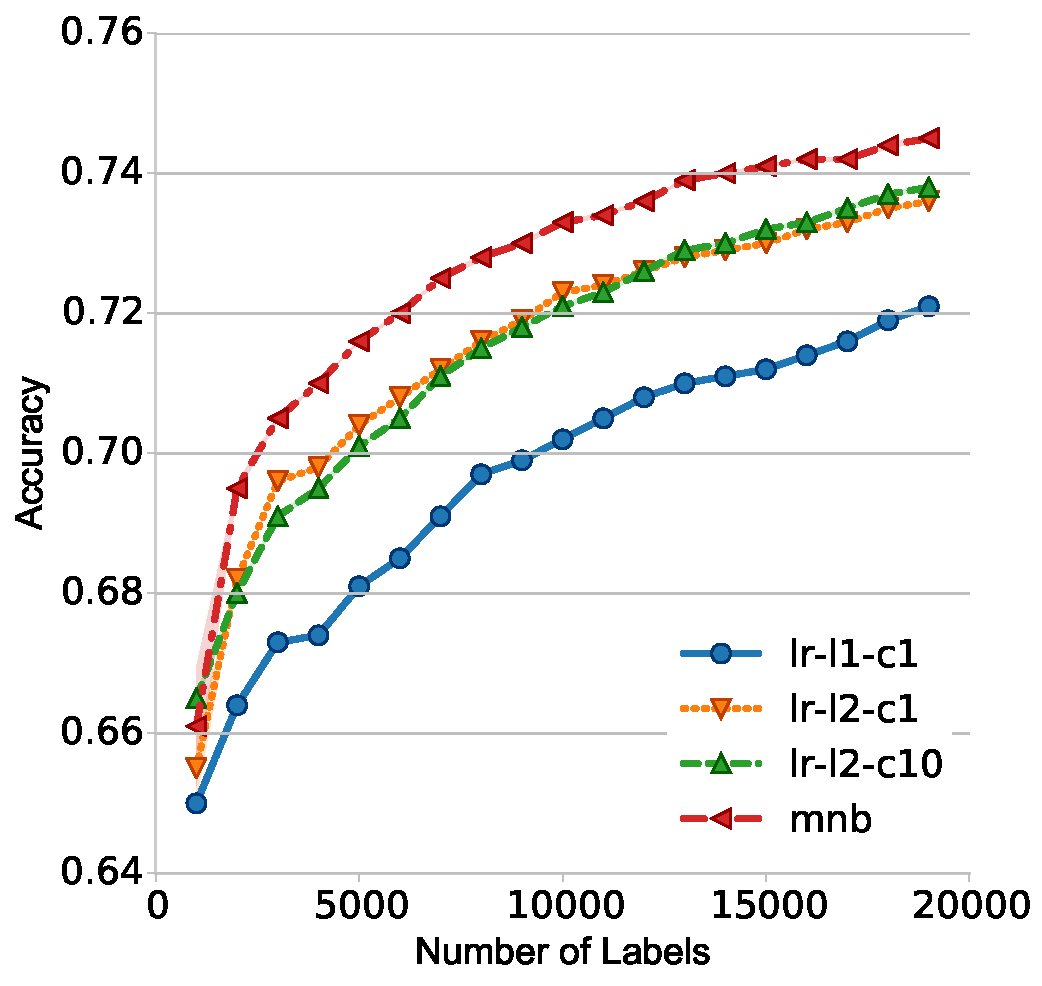
\includegraphics[width=0.9\columnwidth]{fig/models-accu.pdf}
			\label{fig:class}	
%			}	
		}
		\vskip -0.15in
		\caption{Classification models induced on tweets. The performance of four probabilistic classifiers on tweeter data. The budget is the number of labels.}
		\label{fig:user}
	%\end{center}
	\vskip -0.1in
\end{figure*}

\subsection{Data Representation}

We set to find an appropriate data feature vector representation. We tested three data processing options: lower case, URL and mention collapse. We tried all eight combinations and tested using a five fold cross validation. In average, the accuracy of the classifier is 82.5\% ($+/-$ 0.4). We observed that there are no significant differences among all variations, we use the combination of all options active to reduce the size of the dictionary. 

%\subsection{Classification of Individual Tweets}
%\begin{figure*}[t]
%	%\vskip -0.2in
%	%\begin{center}
%	\centering
%		\centerline{
%			\subfigure[IMDB ]{
%				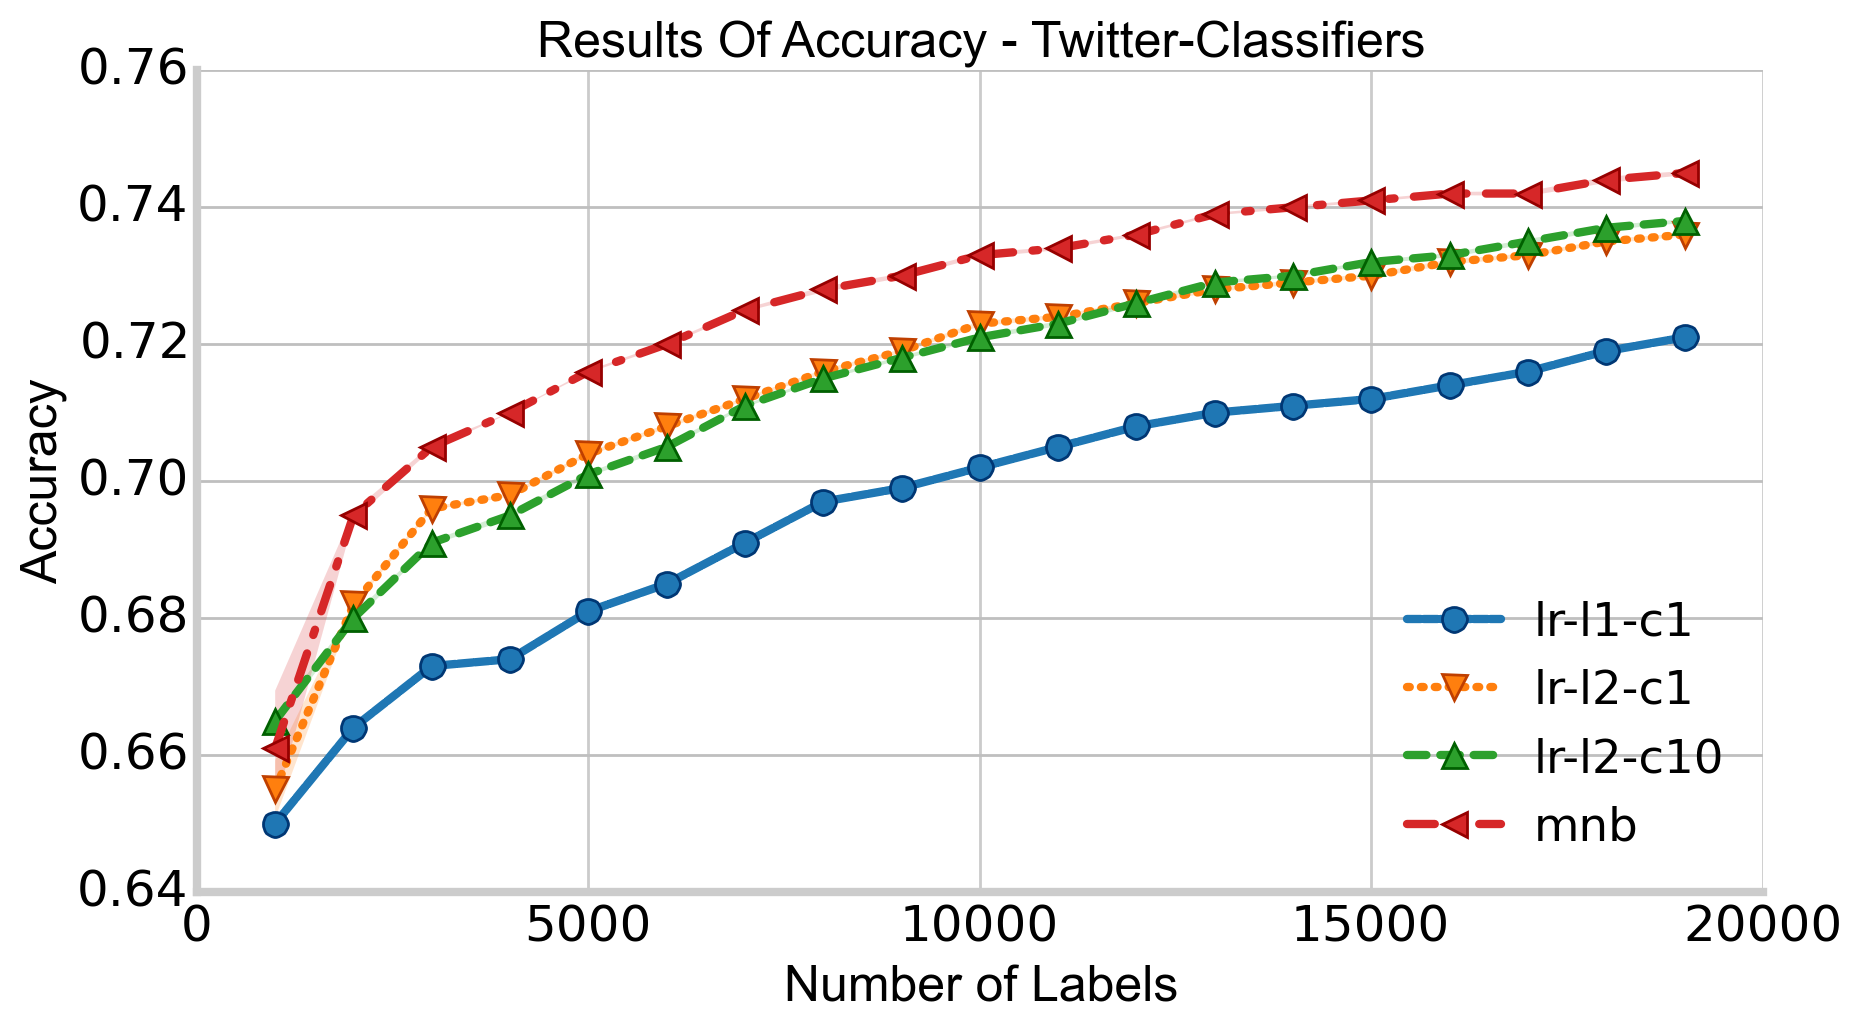
\includegraphics[width=0.7\columnwidth]{fig/twitter-classifiersaccuracy.png}
%			\label{fig:class}	
%			}	
%		}
%		\vskip -0.15in
%		\caption{Classification models induced on tweets.}
%		\label{fig:user}
%	%\end{center}
%	\vskip -0.1in
%\end{figure*}
%
%\begin{figure*}[t]
%	%\vskip -0.2in
%	%\begin{center}
%	\centering
%			\subfigure[IMDB ]{
%				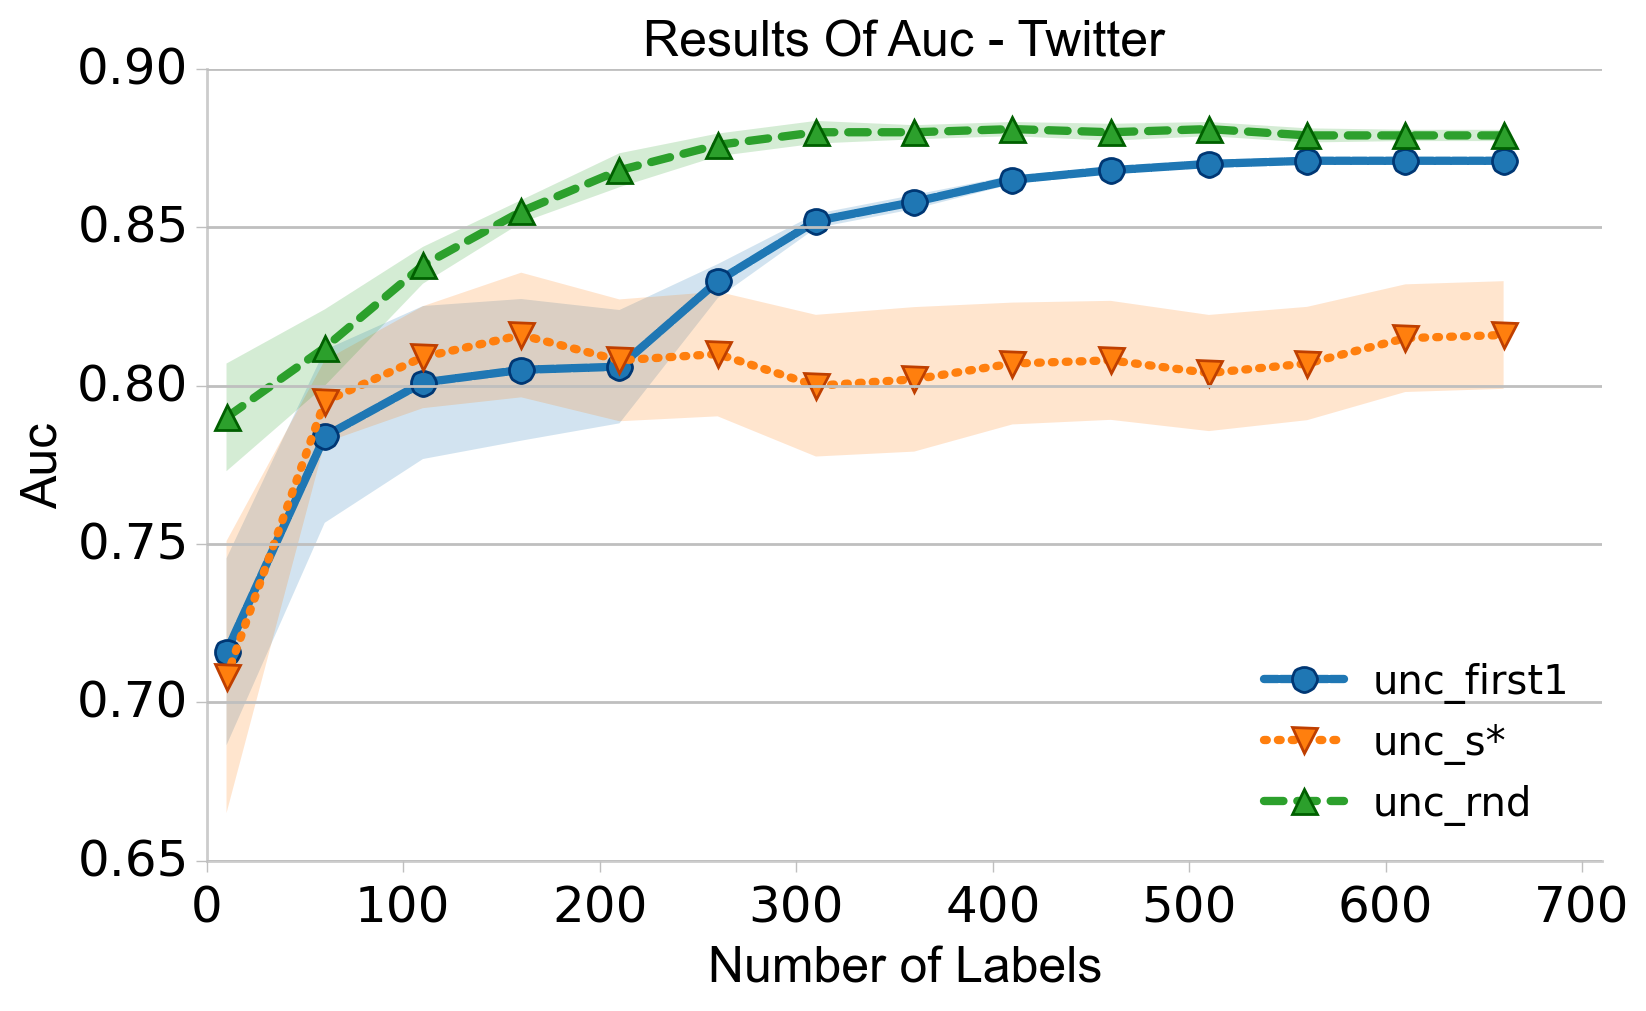
\includegraphics[width=0.7\columnwidth]{fig/twitterauc.png}
%			\label{fig:class}	
%			}	
%		\vskip -0.15in
%		\caption{Active Learning.}
%		\label{fig:user}
%	%\end{center}
%	\vskip -0.1in
%\end{figure*}

\subsection{Other Features}
We tested the use of other features derived from the text such uniqueness of the terms. For example, a bot may use the same terms over and over thus the number unique terms will be low. The uniqueness formulations was: 
%
\begin{equation}
Unique(\x_i) = \frac{TF}{UniqueTerms}
\end{equation}
%
\noindent where $TF$ is the term frequency. We tested this feature representation and obtained 54\% accuracy (+/-0.0). We conjecture that the difference of this measure between the two classes is not significant to have enough classification power. 

\subsection{Error Analysis}
We analyzed a fully trained classifier and reviewed the mistakes made on a test split. The idea is to identify if the classifier is able to reasonable annotate individual tweets, from a human point of view. We used a {\tt{lr-l2-c1}} and we verify the incorrect labels with high incorrect probability. We found that the classifier usually mislabels tweets in other languages other than english, due to low number of examples. Common mistakes, also occurred on tweets with only mentions and URLs. \tabref{tab:twmistakes} show examples of mistakes made by the classifier. 

\begin{table*}[htdp]
\begin{center}
\begin{tabular}{|p{5cm}|c|l|}
\hline \textbf{Tweet Example} & \textbf{True Label} & \textbf{Observation} \\ \hline
THIS\_IS\_A\_MENTION THIS\_IS\_A\_MENTION  otro ,\textbf{que} a lo mejor no sabe que es la udef & Bot & Other languages \\ \hline
THIS\_IS\_A\_MENTION ?effective \textbf{sales} and \textbf{marketing} is getting to the truth as quickly as possible? \#sales \#marketing \#cmworl   & Human & Terms used \\ \hline
rt THIS\_IS\_A\_MENTION \#goroyals  & Bot & Only mention \\ \hline
\end{tabular}
\caption{Example tweets incorrectly labeled by a {\tt{lr-l2l-c1}} classifier. The terms in bold face correspond to the highest weight value according to the classifier.  }
\end{center}
\label{tab:twmistakes}
\end{table*}%
 

\subsection{Active Learning Experiments}
We tested several method of active learning where the learner algorithm picks a tweet from the timeline of a user and requests the label. We tried several approaches as follows:
\begin{description}
\item[\unc{first1}] is a joint formulation of uncertainty of the timeline and maximum first tweet approach. This is a baseline. 
\item[\unc{rnd}] is a joint formulation of uncertainty  of the timeline and a random tweet. This is a baseline
\item[\unc{sr}] is a joint formulation of uncertainty and the best tweet. We tested using a logistic regression model and a multinomial naive bayes model. 
\end{description}

\figref{fig:sr} shows the results accuracy results of the tested models. We observe that the multinomial naive bayes approach has the worst performance. \unc{first1} and \unc{rnd} are the close in performance, however, selecting random tweets perform slightly better in early iterations. We argue that the oracle responses are imbalanced thus introducing noise in the training data. \tabref{tab:cm-ora} shows the confusion matrix of the oracle after labeling 690 tweets selected by the learning algorithm. Note that \unc{first1} and \unc{rnd} have a balanced percentage of error for both human and bot labels, whereas \unc{sr} mistakenly classifies more tweets as bots. 

\begin{figure*}[t]
	%\vskip -0.2in
	%\begin{center}
	\centering
%			\subfigure[IMDB ]{
				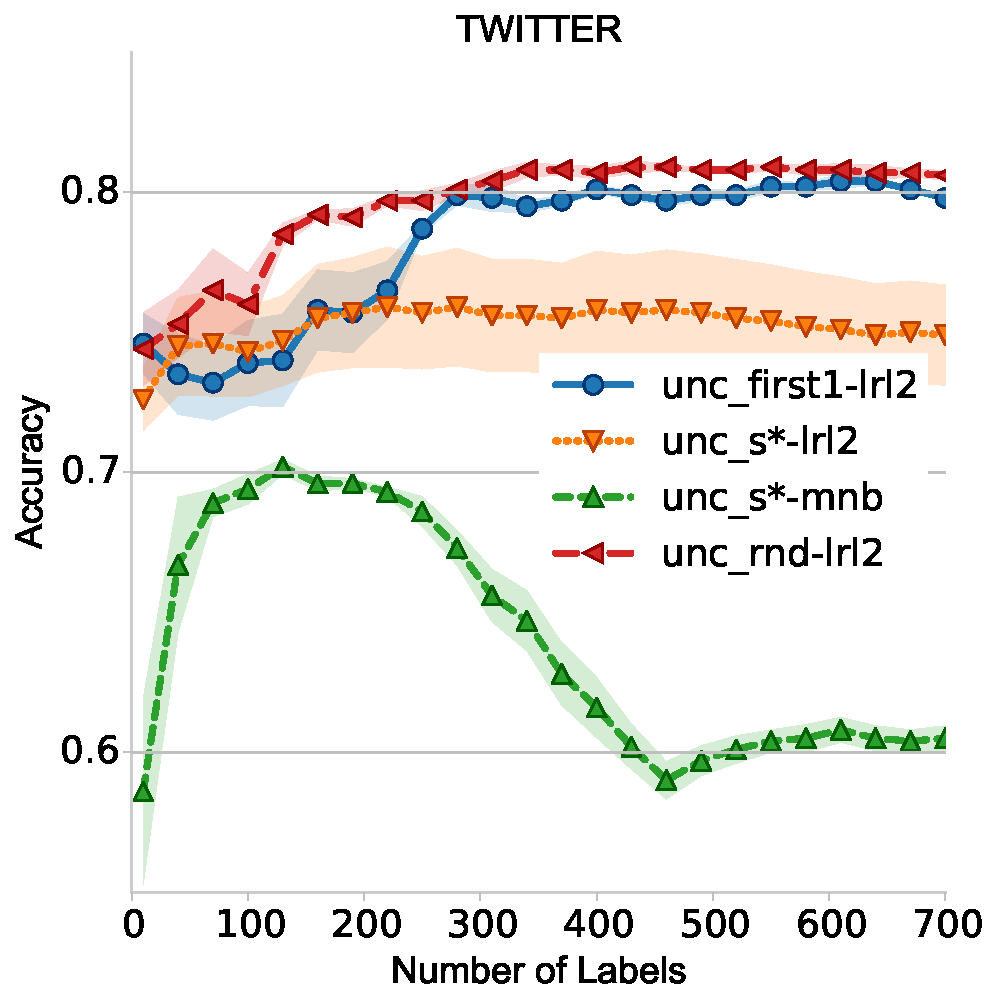
\includegraphics[width=0.9\columnwidth]{fig/sr-accuracy.pdf}
			\label{fig:class}	
%			}	
		\vskip -0.15in
		\caption{Active learning experiments. Results averaged over five trial.}
		\label{fig:sr}
	%\end{center}
	\vskip -0.1in
\end{figure*}

\begin{table*}[!ht]
	%\vskip -0.2in
	\begin{small}
	\begin{center}
		\centering{
			\begin{tabular}{|c|c|c|c|} 
				\multicolumn{4}{c}{\textbf{\unc{first1}-lr}} \\
				\hline \textbf{T. Size }  & & \textbf{H} & \textbf{B} \\ \hline
				690 	&\textbf{H	}	& 40 	& 12 \\ \cline{2-4}
				 	& \textbf{B	}	&12 	& 36 \\ \hline
			\end{tabular} \quad
			\begin{tabular}{|c|c|c|c|} 
				\multicolumn{4}{c}{\textbf{\unc{sr}-lr}} \\
				 \hline \textbf{T. Size }  & & \textbf{H} & \textbf{B} \\ \hline
				690 	&\textbf{ H}	& 35 	& 19 \\ \cline{2-4}
				 	&\textbf{ B	}& 8 	& 39 \\ \hline
			\end{tabular} \quad
			\begin{tabular}{|c|c|c|c|} 
				\multicolumn{4}{c}{\textbf{\unc{sr}-mnb}} \\
				 \hline \textbf{T. Size }  & & \textbf{H} & \textbf{B} \\ \hline
				690 	& \textbf{H}	& 31 	& 23 \\ \cline{2-4}
				 	& \textbf{B}	& 8 	&38 \\ \hline
			\end{tabular}
			\begin{tabular}{|c|c|c|c|} 
				\multicolumn{4}{c}{\textbf{\unc{rnd}}} \\
				 \hline \textbf{T. Size }  & & \textbf{H} & \textbf{B} \\ \hline
				690 	& \textbf{H}	& 40 	& 10 \\ \cline{2-4}
				 	& \textbf{B}	& 11 	& 39 \\ \hline
			\end{tabular}
			}
			\caption{Oracle confusion matrix for different calibration methods on the Twitter dataset. The matrix is given in percentage with respected to the training size (\textbf{T.Size}). \textbf{H} are human labels and \textbf{B} are bot labels. Each row are true labels and columns are predicted by the classifier. }
		\label{tab:cm-ora}
		\vskip -0.25in
	\end{center}
	\end{small}
\end{table*}


\subsection{Other models and Bootstrap Effect}

An important element of the active learning strategy is the bootstrap size of the training data. Bootstrap size can affect how good are the decision of the learner at early iterations. We tested sizes $bt \in \{10, 50, 100\}$ using \SR\ approaches and a logistic regression with L2 regularizations. \figref{fig:bt} shows the learning curve of the methods with different bootstrap sizes. We observe that the differences are not significant (note the standard error per method, i.e., shadowed in the graph), however, the smallest bootstrap is worse than using 100 user timelines. 

\begin{figure*}[t]
	\centering{
			\subfigure[Bootstrap Effect ]{
				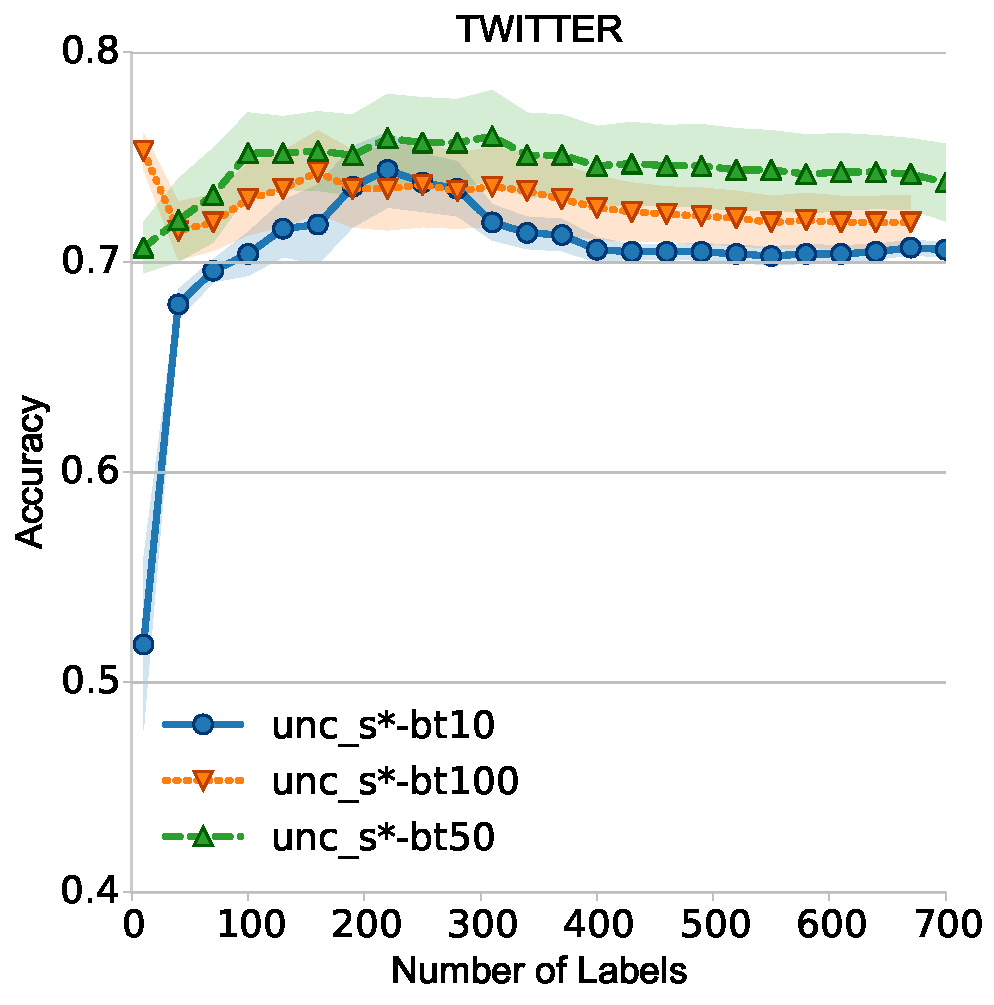
\includegraphics[width=0.8\columnwidth]{fig/bt-accuracy-twitter.pdf}
			\label{fig:bt}	
			} \quad		
			\subfigure[Adaptive Penalty ]{
				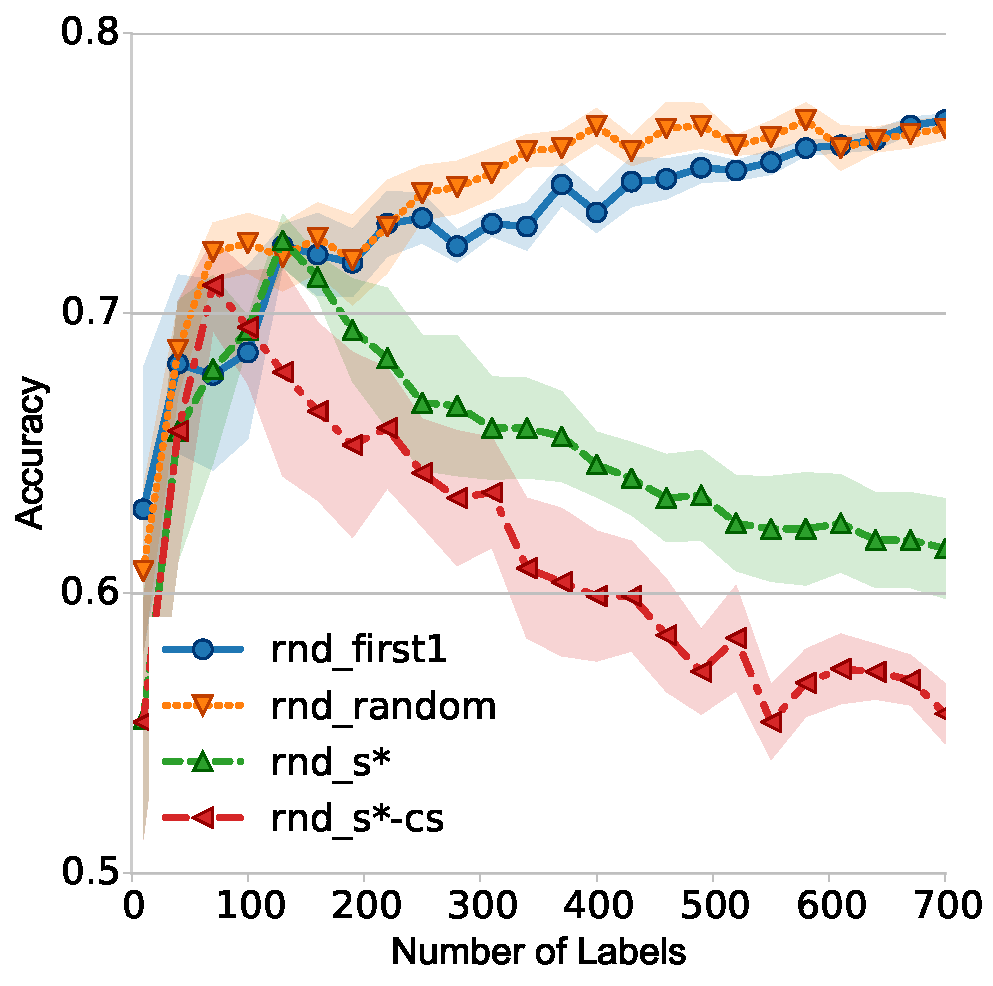
\includegraphics[width=0.8\columnwidth]{fig/lradapt-accuracy-twitter.pdf}
			\label{fig:penalty}	
			}	
		}
		\vskip -0.15in
		\caption{Effect of penalty and bootstrap on the \SR\ methods}
	\vskip -0.1in
\end{figure*}

We also wanted to test if a fixed penalty for the logistic regression model can improve the performance of our proposed method. \figref{fig:penalty} shows the effect of changing the penalty of the model as the training data also changes. We used a random sampling method to isolate the effect of the penalty on the tweet selecting. We observed that the effect of the change does not improve the \SR\ methods to be comparable with the random and first1 baseline. 